 \documentclass[10pt, twocolumn]{IEEEtran}
\usepackage{amsfonts, amsmath, amssymb, epsfig, graphicx}

\newcommand{\n}{\noindent}
\newcommand{\field}[1]{\mathbb{#1}}
\newcommand{\D}[2]{\frac{\partial #2}{\partial #1}}
\newtheorem{theorem}{Theorem}
\newtheorem{lemma}[theorem]{Lemma}
\newtheorem{corollary}[theorem]{Corollary}
\newtheorem{definition}{Definition}
\newcommand{\thmend}{\hspace*{\fill}~\QEDopen\par\endtrivlist\unskip}
\newcommand{\eqdef}{ \stackrel{\bigtriangleup}{=} }
\newcommand{\e}{\epsilon}
\oddsidemargin  0.0in \evensidemargin 0.0in \textwidth      6.25in
\headheight     0.0in \topmargin      0.0in \textheight 9.25in
%\allowdisplaybreaks[4]
 % peanut gallery comments
%
%
% NOTE: Comment *in* the line below if you want a draft with no red comments.
% NOTE: Doing so may replace some of the red comments with 
%       extra spaces or newlines.
%\def\noeditingmarks{}
%
\newcommand{\textred}[1]{\textcolor{red}{#1}}
\ifx\noeditingmarks\undefined
  \newcommand{\pgwrapper}[2]{\textred{#1: #2}}
\else
  \newcommand{\pgwrapper}[2]{}
\fi


\begin{document}

\title{Information Theory in Economics and Investment}
\author{Preston Hansen\\
{\it University of Illinois at Chicago} \\
E-mail: phanse4@uic.edu}
\maketitle

\begin{abstract}
\end{abstract}

\section{Introduction}

Big results in information theory applied to economics and investing. Hopefully a look at open problems.

\section{Information Theory in Economics}

\subsection{Rational Inattention - Modeling behavior in the absence of perfect information}
Discuss rational inattention (especially in the context of typical models of behavior in economics).

Also discuss results and newer papers.
\subsection{Robustness}
Similar motivation to rational inattention.

Again discuss results and newer papers.
\subsection{Credit Risk Modeling}
Info theory used to develop AIC - used in all sorts of model validation.

One paper also uses AIC to look at the predictability of the stock market historically.
\section{Information Theory in Investment}
Lots and lots of papers by Cover on this stuff.
\subsection{Value of Information}
\subsection{Influence of Side Information in Investment}
\subsection{Cost of Achieving the Best Portfolio in Hindsight}


%You can include figures such as \ref{fig:owl}  in .eps, .jpg, .pdf format like this:

% \begin{figure}[h]
% 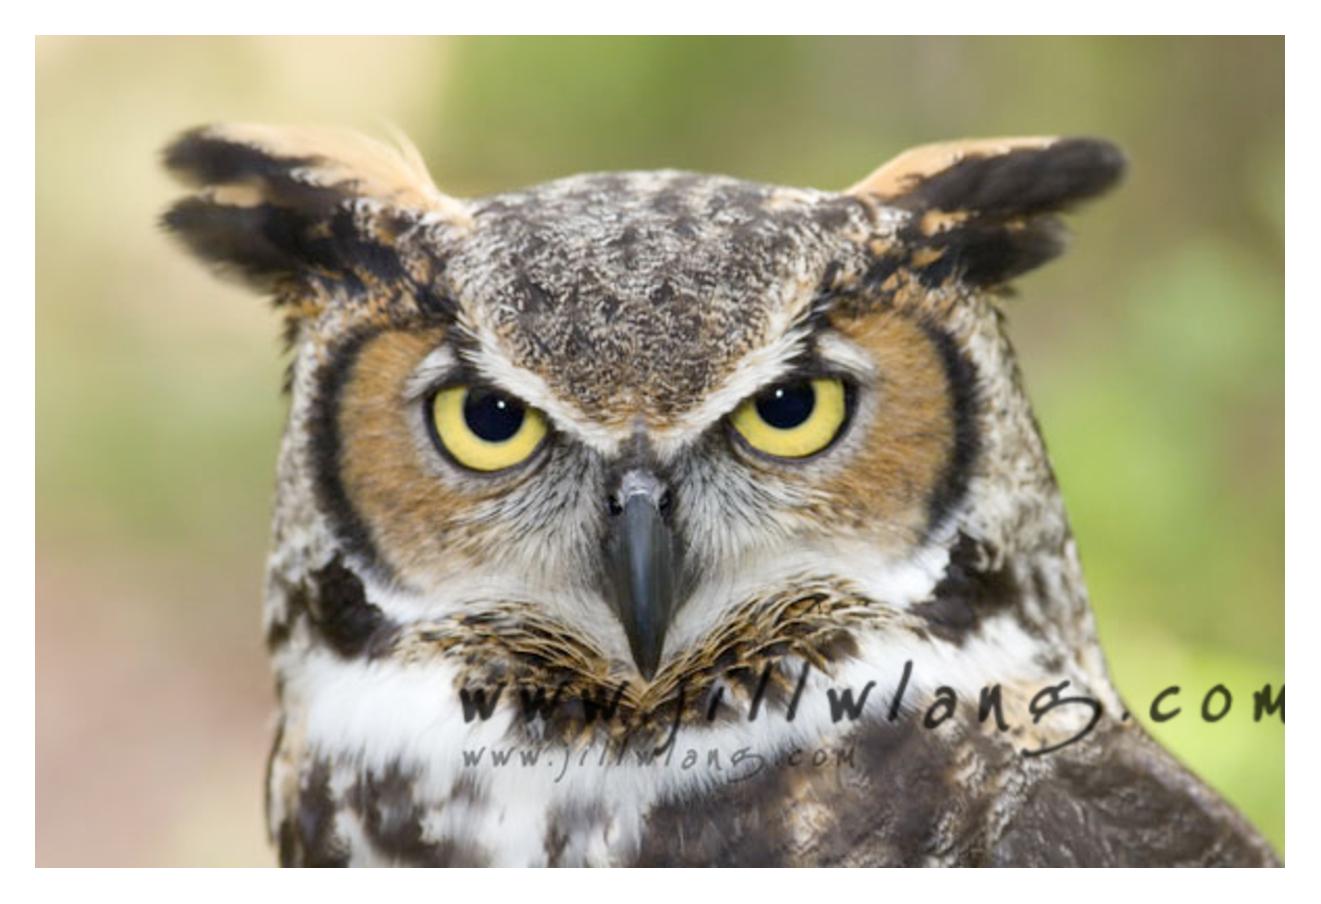
\includegraphics[width=8cm]{owl}
% \centering \caption{Great horned owls are great.}
%  \label{fig:owl}
% \end{figure}

%I can reference files in the {\tt refs.bib}.

running refs list: \cite{RePEc:eee:monchp:3-04}, \cite{Burnham2011}, \cite{Cover2005}, \cite{Cover1988},

\cite{Cover1998}, \cite{Li2017}, \cite{Sims2003}, \cite{Woodford2009}, \cite{Hansen2010}, \cite{StochasticGames},

\cite{Pesaran1995}


 
\baselineskip=2pt
\bibliographystyle{IEEEtrans}
\bibliography{refs}

\end{document}
